\documentclass[french,10pt,twocolumn]{article}
\usepackage[T1]{fontenc}
\usepackage[utf8]{inputenc}
\usepackage{lmodern}
\usepackage[a4paper,top=0.5cm, left=0.5cm, right = 0.5cm, bottom = 0.5cm]{geometry}
\usepackage{amsmath}
\usepackage{tikz}
\usepackage{pgfplots}
\usepackage{subfig}
\usepackage{placeins}
\usepackage{enumerate}
\usepackage{amssymb}
%\usepackage[twocolumn]{multicol}
\usepackage{titling}
%\setlength{\droptitle}{-3cm}	

\usetikzlibrary{calc}
\usetikzlibrary{decorations.markings}
\usetikzlibrary{angles,quotes} % for pic
\usetikzlibrary{arrows.meta} % for arrow size
\usetikzlibrary{bending} % for arrow head angle
\usetikzlibrary{decorations.pathmorphing} % for decorate random steps
\tikzset{>=latex} % for LaTeX arrow head

\def\spaceans{\underline{\hspace{1cm}}}
\def\spaceTF{$\big(\quad\big)$}

%\input{./styles_OMP}
\definecolor{monOrange}{RGB}{255,157,0}
\tikzset{vecteur/.style={->,thick,color=black,smooth}}
\tikzset{force/.style={->,ultra thick,rounded corners=4pt,color=monBleu,smooth,line cap=round}}
\definecolor{monBleu}{rgb}{0.2,0.4,0.6}

\title{\vspace{-1cm} \large $1^{er}$ Contrôle Continu de Mécanique du Point 2 (13/03/2024) - 	Faculté de Sciences et Technologie - UPEC \\ 	Responsable TD: Felipe FIGUEREDO ROCHA (\texttt{felipe.figueredo-rocha@u-pec.fr}) \\
	NOM:\underline{\hspace{7cm}} Prénom: \underline{\hspace{5cm}}  Numéro: \underline{\hspace{2cm}} \\
	Licence:\underline{\hspace{7cm}} Groupe: \underline{\hspace{5cm}} Note: \underline{\hspace{1.5cm}}
	\vspace{-2cm}}
\author{}
\date{}
\begin{document}
	\maketitle
	
	\vspace{-0.5cm}
	\subsection*{Rappels (regarder le tableau aussi)}
	\begin{itemize}
		\item Calculettes et téléphones \textbf{interdits}.
		\item N'oubliez vos noms en toutes les feuilles, les unités, des flèches au-dessus des vecteurs, etc.
		\item Norme produit vectoriel: |$\vec{a} \wedge \vec{b}| =  \|a\| \|b\| |\sin{\theta}(\vec{a}, \vec{b})|$.
		\item Si $(\vec{u}_x, \vec{u}_y, \vec{u}_z)$ est dite une base orthonormé direct, on a: $\vec{u}_x \wedge \vec{u}_y = \vec{u}_z$, $\vec{u}_y \wedge \vec{u}_z = \vec{u}_x$, $\vec{u}_z \wedge \vec{u}_x = \vec{u}_y$.
		\begin{figure}[h!]
			\centering
			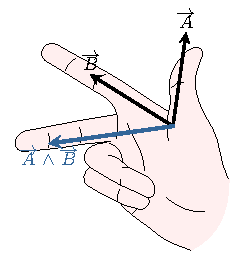
\includegraphics[width=0.3\linewidth]{regle_de_la_main_droite}
			\caption*{}
			\label{fig:regledelamaindroite}
		\end{figure}
		\vspace{-1cm}
		\item Repère polaire:
		$ \begin{cases}
			\vec{u}_r &= \cos{\theta} \Vec{u}_x + \sin{\theta} \Vec{u}_y,\\ 
			\vec{u}_{\theta} &= -\sin{\theta} \vec{u}_x + \cos{\theta} \Vec{u}_y
		\end{cases}
		$ 	
		\item Repère de Frénet : $\dot{s} = \|\vec{v}\|$, $\vec{v} = \dot{s} \vec{T}$ et 
		$\vec{a} = \ddot{s} \vec{T} + \dfrac{\ddot{s}}{R} \vec{N}$
		\item Theorème du moment cinétique :
		\begin{align*}
			\frac{d \vec{L}_0}{d t} = \sum \vec{M}_0(\vec{f}), \quad \text{où} \; \vec{L}_0 = \vec{OM}\wedge m\vec{v}, \vec{M}_0(\vec{f}) = \vec{OM}\wedge \vec{f}
		\end{align*}
	\end{itemize}
	
	\FloatBarrier
	
	\subsection*{Q1 Application du produit vectoriel dans la force électromagnétique (8pts)}
	La force électromagnétique appliqué à une particule $M$ de charge $q$, vitesse $\vec{v}$, dans un champs électrique $\vec{E}$ et champs magnétique $\vec{B}$ est donné par $\vec{f}_{EB} = q (\vec{E} + \vec{v} \wedge \vec{B})$. On pose $\vec{f}_E = q \vec{E}$, $\vec{f}_B = \vec{v} \wedge \vec{B}$, tel que $\vec{f}_{EB} = \vec{f}_E + \vec{f}_B$. On va considérer que $q$ est \textbf{négatif} et $\vec{E} = E \vec{u}_x$, $\vec{B} = B \vec{u}_y$, $\vec{v} = v \vec{u}_z$, avec $E, B$ et $v$ nombres \textbf{positifs}. Choisissez $2$ plans entre les $3$ possibilités en repère cartésien ($Oxy$, $Oxz$ ou $Oyz$) pour les questions suivantes. 
	\begin{enumerate}[a)]
		\item Indiquer votre choix dans les cases correspondants et placer le troisième vecteur de la base cartésienne à l'origine cohérent avec votre choix (rappel: $\otimes$ ou $\odot$  sont respectivement un vecteur rentrant ou sortant du plan.) 
		\item Dessiner les vecteurs $\vec{v}$, $\vec{B}$ et $\vec{E}$ (obs: dans les deux plans, la taille des flèches n'est pas important).
		\item Dessiner les vecteurs $\vec{f}_E$ et $\vec{f}_B$ (même observations que b)). 
		\item Donner l'expression de $\vec{f}_{EM}$ en fonction de $q, E, B$ et $v$.
		\item Pour quelle valeur de $v$ (en fonction des autres données), la force $\vec{f}_{EM} = \vec{0}$.
		\item On pose $v_0$ la valeur critique trouvé en e). Dessiner le vecteur $\vec{f}_{EM}$ pour $v>v_0$ (même observation que b)).
		\item Calculer le moment de $\vec{f}_{EB}$ par rapport a $O$ quand la particule se trouve dans la position générique $\vec{OM} = a\vec{u}_x + b\vec{u}_y + c\vec{u}_z$.
	\end{enumerate}
	
	\begin{figure}[h!]
		\centering	
		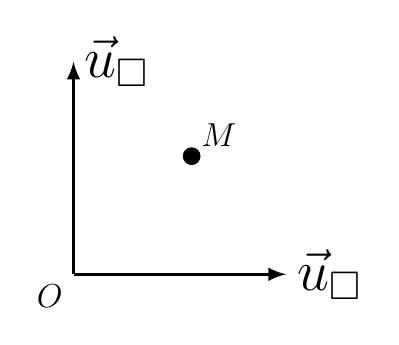
\begin{tikzpicture}[scale=1.5]
			\coordinate (O) at (0,0);
			\coordinate (X) at (1.8,0);
			\coordinate (Y) at (0,1.8);
			\coordinate (M) at (1.0, 1.0);	
			\draw[very thick,->] node[below left]{\large $O$} (O)--(X) node[right]{\huge $\vec{u}_{\square}$};
			\draw[very thick,->](O)--(Y) node[right]{\huge $\vec{u}_{\square}$};
			\filldraw[black] (M) circle (2pt) node[anchor=south west]{\large $M$};
		\end{tikzpicture}
		\hfill
		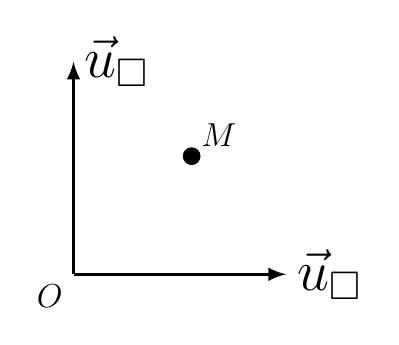
\begin{tikzpicture}[scale=1.5]
			\coordinate (O) at (0,0);
			\coordinate (X) at (1.8,0);
			\coordinate (Y) at (0,1.8);
			\coordinate (M) at (1.0, 1.0);	
			\draw[very thick,->] node[below left]{\large $O$} (O)--(X) node[right]{\huge $\vec{u}_{\square}$};
			\draw[very thick,->](O)--(Y) node[right]{\huge $\vec{u}_{\square}$};
			\filldraw[black] (M) circle (2pt) node[anchor=south west]{\large $M$};
		\end{tikzpicture}
		\caption*{}
		\label{fig:plan_xz}
	\end{figure}
	\vspace{-1cm}	
	\FloatBarrier
	\vspace{-1cm}
	\subsection*{Q2 : Un esquimau sur un igloo (12pts)} 
	L’enfant se laisse glisser avec frottement $\vec{f}$ (avec sa norme noté par $f$) depuis le sommet de l’igloo qui a la forme d’une demi-sphère de rayon $R$ et de centre $O$. La position de l'enfant, assimilé à un point matériel $M$ de masse $m$ est repérée par l’angle $\theta$ par rapport à $\vec{u}_x$ (augmentant un direction à $\vec{u}_y$) . La norme de l'accéleration de la pesanteur est dénoté $g$, tel $\vec{g} = -g\vec{u}_y$ point vers le bas. L'objectif de cet exercice est d'étudier le mouvement en repère de \textbf{Frénet}. 
	\begin{enumerate}[a)]
		\item(1,0pt) Complétez la figure ci-dessous en plaçant $\vec{T}$ (supposant $\dot{\theta}>0$), $\vec{N}$ et $\vec{B}=\vec{T}\wedge \vec{N}$ (Obs: ($\vec{T}$, $\vec{N}$, $\vec{B}$) forme un base orthonormée direct).
		\begin{figure}[h!]
			\centering
			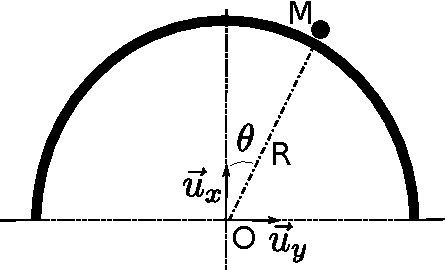
\includegraphics[width=0.5\linewidth]{igloo}
			\caption*{}
		\end{figure}
		\vspace{-1cm}
		\item(1,5pt) Donner les expressions de toutes les forces en repère de Frénet.
		\item(1,5pt) Calculer les moments de chacune de ces forces par rapport au point $O$.
		\item(1,5pt) Calculer le moment cinétique de l'enfant par rapport au point $O$.
		\item(1,5pt) Appliquer le théorème du moment cinétique à ce mouvement.
		\item(1,5pt) Appliquer le principe fondamentale de la dynamique (PFD) projeté sur le vecteur normale du repère de Frénet.
		\item(2,0pt) On va supposer que $f = \alpha R_N$ ($\alpha >0$ un coefficient donné). Trouver une équation différentielle unique avec les résultats des exercises e) et f).
		\item(1,5pt) Expliquer la différence principale entre le vecteur $\vec{T}$ en repère de Frénet et de  $\vec{u}_{\theta}$ dans le repère cylindrique. Quel est l'intérêt de l'utilisation du repère Frénet pour modéliser le frottement par rapport l'utilisation du repère cylindrique. 
	\end{enumerate}
\end{document}
